%-------------------------
% Resume in Latex
% Author : Zakaria TOZY
%------------------------

\documentclass[11pt,a4paper]{article}

\usepackage{latexsym}
\usepackage[empty]{fullpage}
\usepackage{titlesec}
\usepackage{marvosym}
\usepackage[usenames,dvipsnames]{color}
\usepackage{verbatim}
\usepackage{enumitem}
\usepackage[hidelinks]{hyperref}
\usepackage{fancyhdr}
\usepackage[english,french]{babel}
\usepackage{tabularx}
\usepackage[utf8]{inputenc}
\usepackage[left=0.5in, right=0.5in, top=0in, bottom=0in]{geometry}
\usepackage{exscale}  % Pour la commande \HUGE

\usepackage{fontawesome}
\usepackage[scale=0.90,lf]{FiraMono}

\definecolor{light-grey}{gray}{0.83}
\definecolor{dark-grey}{gray}{0.3}
\definecolor{text-grey}{gray}{.08}

\DeclareRobustCommand{\ebseries}{\fontseries{eb}\selectfont}
\DeclareTextFontCommand{\texteb}{\ebseries}

\usepackage{contour}
\usepackage[normalem]{ulem}
\renewcommand{\ULdepth}{1.8pt}
\contourlength{0.8pt}
\newcommand{\myuline}[1]{%
  \uline{\phantom{#1}}%
  \llap{\contour{white}{#1}}%
}

\usepackage{tgheros}
\renewcommand*\familydefault{\sfdefault} 
\usepackage[T1]{fontenc}

\usepackage{graphicx}

\pagestyle{fancy}
\fancyhf{} 
\fancyfoot{}
\renewcommand{\headrulewidth}{0pt}
\renewcommand{\footrulewidth}{0pt}

\urlstyle{same}

\raggedbottom
\raggedright
\setlength{\tabcolsep}{0in}

\titleformat{\section}{
    \bfseries \vspace{-4pt} \raggedright \normalsize
}{}{0em}{}[\color{light-grey} {\titlerule[1pt]} \vspace{-2pt}]

\newcommand{\resumeItem}[1]{
  \item\footnotesize{
    {#1 \vspace{-1pt}}
  }
}

\newcommand{\resumeSubheading}[4]{
  \vspace{2pt}\item
    \begin{tabular*}{\textwidth}[t]{l@{\extracolsep{\fill}}r}
      {\footnotesize\textbf{#1}} & {\footnotesize#2} \\
      {\footnotesize\textit{#3}} & {\footnotesize\textit{#4}} \\
    \end{tabular*}\vspace{2pt}
}

\newcommand{\resumeProjectHeading}[2]{
  \item
  {\footnotesize\textbf{#1}} \hfill {\footnotesize\textit{#2}}
}

\newcommand{\resumeSubItem}[1]{\resumeItem{#1}\vspace{-4pt}}

\renewcommand\labelitemii{$\vcenter{\hbox{\tiny$\bullet$}}$}

\newcommand{\resumeSubHeadingListStart}{\begin{itemize}[leftmargin=0in, label={}]}
\newcommand{\resumeSubHeadingListEnd}{\end{itemize}}
\newcommand{\resumeItemListStart}{\begin{itemize}[label={\textbullet}]}
\newcommand{\resumeItemListEnd}{\end{itemize}\vspace{0pt}}

\color{text-grey}

\begin{document}

\begin{flushleft}
  \begin{minipage}[c]{0.2\textwidth}
    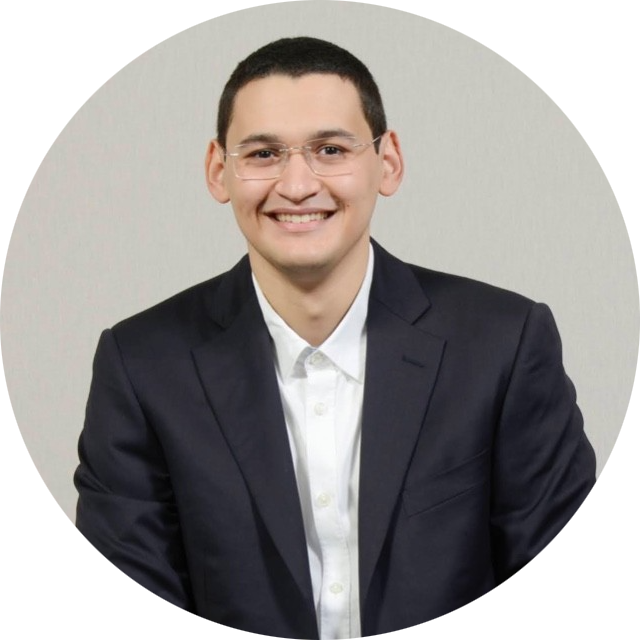
\includegraphics[width=3cm]{images/profilpicture.png}
  \end{minipage}%
  \begin{minipage}[c]{0.8\textwidth}
    {\Huge \textbf{Zakaria TOZY}} \\[2pt]
    {\Large \textbf{Data Engineer | CDI}}
  \end{minipage}
\end{flushleft}

\vspace{-25pt}

\begin{center}
    \small \faPhone\ \texttt{0617407077} \hspace{1pt} $|$
    \hspace{1pt} \faEnvelope\ \texttt{zakaria.tozy@icloud.com} \hspace{1pt} $|$
    \hspace{1pt} \faLinkedin\ \texttt{zakaria-tozy} \hspace{1pt} $|$
    \hspace{1pt} \faMapMarker\ \texttt{Paris} \hspace{1pt} $|$
    \hspace{1pt} \faGithub\ \texttt{zack242} \\ \vspace{0pt}
\end{center}

\begin{itemize}[leftmargin=0in, label={}]
\footnotesize{\item{
Jeune ingénieur diplômé d'un double cursus en systèmes d'information et data science, avec une forte passion pour la data, l'IA et les nouvelles technologies. Je resors fort d'une expérience en tant que Data Engineer / Data analyst au sein de AXA IM, et je suis à la recherche d'un CDI pour mettre en pratiques mes competences.
}}
\end{itemize}

\section{COMPETENCES}
\begin{itemize}[leftmargin=0in, label={}]
\footnotesize{\item{
{\footnotesize\textbf{Programmation}:} {\footnotesize Python, SQL, Java, JavaScript} \\
\vspace{3pt}
{\footnotesize\textbf{Machine Learning}:} {\footnotesize Scikit-Learn, Pandas, Numpy, NLP, LLM} \\
\vspace{3pt}
{\footnotesize\textbf{Devops}:} {\footnotesize Docker, CI/CD, Git} \\
\vspace{3pt}
{\footnotesize\textbf{Soft Skills}:} {\footnotesize Autonome, Rigoureux, Esprit d'analyse, Apprentissage rapide} \\
\vspace{3pt}
{\footnotesize\textbf{Langues}:} {\footnotesize Français (Bilingue), Arabe (Bilingue), Anglais (Courant - TOEIC 875)} \\
\vspace{3pt}
{\footnotesize\textbf{Data \& Cloud Engineering}:} {\footnotesize PySpark, Databricks,Snowflake, Azure,GCP,S3, dbt}
}
}
\end{itemize}

\section{FORMATIONS}
\resumeSubHeadingListStart
    \resumeSubheading
      {École Centrale d'Électronique (ECE Paris)}
      {Janvier 2024}
      {Ingénieur en Systèmes d'Information et Big Data Analytics}
      {Top 5\% de la promotion}
      \resumeItemListStart
        \resumeItem{Spécialisation : Programmation, Bases de données, Électronique}
      \resumeItemListEnd
    \resumeSubheading
      {Institut Polytechnique de Paris (École Polytechnique)}
      {Janvier 2024}
      {Master 2 en Data Sciences}
      {Mention Très bien}
      \resumeItemListStart
        \resumeItem{Spécialisation : Machine Learning, Big Data, Cloud Infrastructure, Deep Learning, NLP}
      \resumeItemListEnd
  \resumeSubHeadingListEnd

\section{EXPERIENCES}
\resumeSubHeadingListStart
    \resumeSubheading
      {Projet Personnel}{Février 2024 --- Juin 2024}
      {Ingénieur Blockchain - Dévellopement d'un sniper bot en Rust}{Paris}
      \resumeItemListStart
        \resumeItem{Monitoring de tous les tokens créés sur la blockchain Solana}
        \resumeItem{Mise en place d'un système pour acheter ces tokens dès leur création en moins de 1s}
        \resumeItem{Vente automatique des tokens après réalisation d'une plus-value}
      \resumeItemListEnd
    \resumeSubheading
      {AXA Investment Managers - AXA IM}{Août 2023 --- Janvier 2024}
      {Stage de Fin d'Études - Data Engineer / Data Analyst}{Paris}
      \resumeItemListStart
        \resumeItem{Conception et mise en place de pipelines de données pour l'ingestion et la gestion des données métiers}
        \resumeItem{Optimisation du modèle de données et migration des pipelines de distribution pour le reporting financier de 844 milliards d'euros d'actifs}
        \resumeItem{Tests de nouveaux clusters Databricks et création d'un PoC pour l'anonymisation des données sensibles}
        \resumeItem{Création de tableaux de bord et calcul des KPIs pour la vision distribuée (ME, OV, CIS, FX)}
      \resumeItemListEnd
    \resumeSubheading
      {Kalima Blockchain et IoT}{Avril 2022 --- Août 2022}
      {Stage - Software Engineer}{Paris}
      \resumeItemListStart
        \resumeItem{Développement d'un explorateur de blockchain propriétaire Kalima en Java/LevelDB (+1000 transactions par seconde)}
        \resumeItem{Implémentation de nouvelles fonctionnalités d'administration pour la blockchain propriétaire Kalima en Node.js}
        \resumeItem{Conception et développement d'un système d'authentification multisignature pour les DApps (Decentralized Applications)}
      \resumeItemListEnd
    \resumeSubheading
      {Le Crédit Lyonnais - LCL}{Janvier 2020 --- Février 2020}
      {Stage - IT Support}{Paris}
      \resumeItemListStart
        \resumeItem{Étude de migration Microsoft Office 2010 vers 2016 et analyse de son impact sur les processus métiers}
        \resumeItem{Développement et exécution de procédures de tests sur un parc de 23 000 postes de travail}
      \resumeItemListEnd
  \resumeSubHeadingListEnd

\section{PROJETS}
\resumeSubHeadingListStart
    \resumeProjectHeading
      {Bitcoin Analysis} {Août 2024}
      \resumeItemListStart
        \resumeItem{Création d'un pipeline de données avec Python, SQL, Airflow, dbt et Snowflake pour l'analyse des transactions Bitcoin, traitant plus de 1 million de transactions par jour.}
      \resumeItemListEnd
    \resumeProjectHeading
      {Twitter Real-time Analysis} {Avril 2023}
      \resumeItemListStart
        \resumeItem{Développement d'un système de visualisation en temps réel des flux Twitter par sujets à l'aide de Kafka et de l'algorithme KNN (K-Nearest Neighbors).}
      \resumeItemListEnd
    \resumeProjectHeading
      {Agent AI Autonome} {Novembre 2024}
      \resumeItemListStart
        \resumeItem{Développement d'un agent AI autonome utilisant le framework ai16z}
        \resumeItem{Deploiment de l'agent ai sur Twitter dans le but d'interagir avec les utilisateurs}
        \resumeItem{Utilisation de l'api de open ai pour la génération de réponses}
      \resumeItemListEnd
\resumeSubHeadingListEnd


\end{document} 